\documentclass[12pt,a4paper]{article}

\usepackage[utf8]{inputenc}
\usepackage[greek,english]{babel}
\usepackage{float}
\usepackage[export]{adjustbox}
\usepackage{sans}
\usepackage{kerkis} 
%\usepackage{sans}
%\usepackage[LGRgreek]{mathastext}   
\usepackage{graphicx}
\usepackage{enumerate}
%\usepackage{enumitem}  
\usepackage{amsmath}
\usepackage{hyperref,xcolor} 
\hypersetup{
    colorlinks,
    linkcolor={black!50!black},
    citecolor={blue!50!black}, urlcolor={cyan!80!black},
}

\newcommand{\en}{\selectlanguage{english}} 
\newcommand{\tl}{\textlatin} 
\newcommand{\gr}{\selectlanguage{greek}}   
\newcommand{\code}[1]{\texttt{#1}}         
%\newcommand{\tsuper}{\textsuperscript} \newcommand{\tsub}{\textsubscript}
\renewcommand{\labelenumi}{\alph{enumi}}

 \renewcommand{\thesection}{\arabic{section}.} 
% \renewcommand{\thesubsection}{\arabic{subsection}.}


\gr \title{{\bf 
\includegraphics[scale=1.0]{images/up_landscape.jpg} \\ ΤΜΗΜΑ ΜΗΧΑΝΙΚΩΝ ΗΛΕΚΤΡΟΝΙΚΩΝ ΥΠΟΛΟΓΙΣΤΩΝ ΚΑΙ ΠΛΗΡΟΦΟΡΙΚΗΣ  \\ \vspace{3cm}Αναφορά Εργαστηριακής Άσκησης Μέρος Α' \\ Υπολογιστική Νοημοσύνη}}
\author{Κωνσταντίνος Τσάκωνας}
\date{Ακαδημαϊκό έτος 2020-21\\ Χειμερινό Εξάμηνο}

\begin{document}

    \gr \maketitle \newpage

    \tableofcontents  \newpage

    \section{\tl{Repository} \gr Κώδικα}
        \underline{\tl{\textbf{\url{https://github.com/iamtsac/computational-intelligence-part-a}}}}

    \section{Προεπεξεργασία και Προετοιμασία δεδομένων.} 
    \begin{enumerate}
        \item 
        Το σύνολο των δεδομένων μας αποτελείται από $785$ στήλες. Στην πρώτη στήλη του αρχείου \tl{csv} o περιέχεται αριθμός που απεικονίζεται στην εικόνα, ο οποίος είναι το  \tl{label} για το νερωνικό. Οι υπόπολοιπες στήλες αποτέλουν τα \tl{pixels} της εικόνας. Οπότε το νευρωνικό μας θα έχει ως είσοδο τις στήλες που περιέχουν τα \tl{pixels} και θα εκπαιδευτεί στα δεδομένα του \tl{label}. Στο κώδικα εργαζόμαστε ως εξής, αφού φορτώσουμε τα δεδομένα του \tl{csv(train\_csv)} χρησιμοποιόντας το pandas, χωρίζουμε το \tl{y(label)} από το \tl{x(pixels)}. Στη συνέχεια μετασχηματίζουμε τη λίστα της εισόδου σε ένα ώστε να περιέχει $60.000$ μητρώα $28\times28$ διαστάσεων. Τη παραπάνω εργασία εφαρμόζουμε και στα δεδομένα που έχουμε για τον έλεγχο(\tl{train\_csv}). Μέτα από τα παραπάνω θα προκύψει μια δομή δεδομένων \tl{np.array} διαστάσεων ($6000,28,28$) όπου κάθε θέση θα περιέχει στοιχεία της μορφής:
        \begin{equation*}
        X_i = 
        \begin{bmatrix}
            pixel_{1,1} & pixel_{1,2} & \cdots & pixel_{1,28} \\
            pixel_{2,1} & pixel_{2,2} & \cdots & pixel_{2,n} \\
            \vdots      & \vdots      & \ddots & \vdots  \\
            pixel_{28,1} & pixel_{28,2} & \cdots & pixel_{28,28} 
        \end{bmatrix} 
        \end{equation*}
        \item Για το συγκεκριμένο ερώτημα χώρισαμε τα $60000$ δείγματα σε $5$ κομμάτια. Αφού έγινε ο διαχωρισμός παίρνουμε το κάθε κομμάτι που προκύπτει απο την διάσπαση και κάνουμε επικύρωση με τα υπόλοιπα. Ουσιαστικά χρησιμοποιώντας μία επανάληψη είχαμε σε κάθε εκπαίδευση του μοντέλου $48000$ δεδομένα εκπαίδευσης και $12000$ δεδομένα επικύρωσης. Με αυτό το τρόπο δίνουμε εκπαιδεύουμε το μοντέλο μας σε δεδομένα που δεν έχει ξαναδεί. Κατα αυτόν τον τρόπο μπορούμε να αξιολογίσουμε πως θα ανταποκριθεί το μοντέλο μας σε πργαματικές συνθήκες και μπορούμε επίσης σε περίπτωση που έχουμε να επιλέξουμε μεταξύ αρχιτεκτονικών να συγρκίνουμε τα αποτελέσματα τους από το \tl{Cross-Validation } και να διαλέξουμε την καλύτερη.
    \end{enumerate}

    \section{Επιλογή Αρχιτεκτονικής.}

    \begin{enumerate}
        \item Στο συγκεκριμένο πρόβλημα μπορούμε να αξιολογήσουμε το μοντέλο μας κάνοντας χρήση του \tl{Cross-Entropy} ή του \tl{Mean-Squared-Error}. Το \tl{MSE} αυτό που μας δείχνει για το μοντέλο μας είναι, ότι όσο μικραίνει το \tl{MSE} τόσο πιο κόντα είναι η έξοδο μας στο επιθυμητό αποτέλεσμα. Από την άλλη το \tl{CE} χρησιμποιείται για να κατηγοριοποιήσει το δεδομένα σε κλάσεις. Θα μπορουσε το  \tl{Cross-Entropy} να ερμηνευθεί ως η πιθανότητα να ανήκει η έξοδο του μοντέλου μας σε μία κλάση. Στη περίπτωση μας το \tl{CE} είναι πιο ιδανικό αφού θέλουμε αφού αυτό που εμείς θέλουμε είνα να κατηγοριοποιήσουμε την είσοδο μας σε μία κατηγορία από τις $[0 $-$ 9]$.

        \item Το νευρωνικό μας θα έχει πλήθος εισόδων $ 28^2 = 784 $ δηλαδή όσα είναι και  τα \tl{pixels} σε κάθε εικόνα. Ουσιαστικά με αυτό τον τρόπο δίνουμε στο μοντέλο μας σαν είσοδο μία εικόνα και προσπαθεί να κατηγοριοποιήσει σε μια κλάση. 

        \item Στην έξοδο θα χρειαστούμε 10 νευρώνες.  Αυτό συμβαίνει γιατί θέλουμε η έξοδος του νευρωνικού μας να καθορίζει την κλάση που ανήκει η εικόνα που δώσαμε σαν είσοδο.

        \item Στους κρύφους κόμβους η σανάρτηση ενεργοποίησης που διαλέξαμε είναι η \tl{ReLU}. Η απόφαση για την συνάρτηση του κρυφού επιπέδου είναι αρκετά εύκολη, αρκεί να παρατηρήσουμε την γραφική παράσταση της συνάρτηση και το είδος των δεδομένων. Τα δεδομένα μας είναι εικόνες, από \tl{pixels} οι τιμές των οποίων μέτα το κανονικοποίηση κυμαίνονται στο διάστημα $[0,1]$. Ο τύπος της συνάρτησης \tl{ReLU} είναι ο εξής: 
        $$ f(x)=\max(0,x)$$ 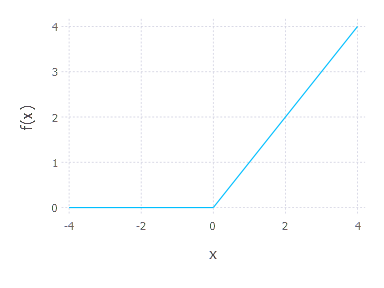
\includegraphics[ height=6cm, center]{images/relu_graph.png} \\ 
        Χρησιμοποιώντας τη \tl{ReLU} πετυχαίνουμε αρκέτα πράγματα εξαιτίας της φύσης του συνόλου δεδομένων που έχουμε. Αρχικά τα δεδομένα είναι αρκετά αραιά, οπότε για κάθε είσοδο δεν θα ενεργοποιούνται όλοι οι νευρώνες, με αποτέλεσμα οι τιμές που δεν προσφέρουν κάποια πληροφορία στο νευρωνικό να μην επηρεάζουν την εκπαίδευση. Επίσης τα μητρώα έχουν τις τιμές που μας ενδιαφέρουν κοντά στο κέντρο, οπότε κατα την πρόοδο της εκπαίδευση θα δούμε μεγάλη βελτιώση αφού θα είναι αρκετά εύκολο για το νευρωνικό να τοποθετήσει τα σωστά βάρη στους κόμβους. Τέλος προσφέρει πολύ μικρή υπλογιστική πολυπλοκότητα στο δίκτυο μας, αφού το μόνο που κάνει είναι απλά μία σύγκριση. 

        \item Στο επίπεδο έξοδου θα χρησιμοποιήσουμε την συνάρτηση \tl{Softmax}, διότι συναρτήσεις όπως  η σιγμοιειδής δεν μπόρει να μας βοηθήσει σε ένα πρόβλημα κατηγοριοποίησης σε περισσότερες από δύο κλάσεις όπως αυτό που έχουμε εδώ.  Αυτό που κάνει η \tl{Softmax} και μας είναι απαραίτητο στο συγκεκριμένο πρόβλημα είναι οτι στη έξοδο συμπικνώνει τις τιμές μεταξύ του διαστήματος $[0-1]$ και το άθροισμα των εξόδων ισούται με $1$. Άρα πρακτικά η συνάρτηση μας δίνει σαν έξοδο την πιθανότητα να ανήκει η είσοδος μας σε κάθε κατηγορία.


        

    \end{enumerate}

\end{document} 